\section{Auswertung}
\label{sec:Auswertung}  

Die Messwerte für die Spannungen von $\SI{150}{\volt}$, $\SI{170}{\volt}$, $\SI{190}{\volt}$, $\SI{210}{\volt}$
und $\SI{240}{\volt}$ sind \autoref{tab:t12}, \autoref{tab:t34} und \autoref{tab:t5} zu finden. Die gemessenen  
Thermistorwiderstände sind im Bereich von $\SI{1,895}{\mega\ohm}$ bis $\SI{1,922}{\mega\ohm}$, so dass nach ... die
Temperatur zu $T\approx \SI{27}{\celsius} = \SI{301,5}{\mega\ohm}$ ablesbar ist. Es wurden nur Tröpfchen untersucht,
die keine Geschwindigkeit ohne angelegtes E-Feld haben, so dass die Messung von $t_{\symup{0}}$ nicht notwendig
ist.
\begin{table}
  \centering
  \caption{Messwerte für $U=\SI{150}{\volt}$ und
  $U=\SI{170}{\volt}$.}
  \label{tab:t12}
  \begin{tabular}{c c c}
    \toprule
    Tröpfchen & $t_{\symup{ab}}/\unit{\second}$ & $t_{\symup{auf}}/\unit{\second}$ \\
    \midrule
    1 & 5,50 & 6,84 \\
      & 5,89 & 7,35 \\
      & 5,54 & 5,70 \\
    2 & 3,89 & 3,71 \\
      & 3,13 & 3,87 \\
      & 3,86 & 5,21 \\
    3 & 2,32 & 2,72 \\
      & 2,99 & 1,81 \\
      & 2,35 & 2,91 \\
    4 & 3,72 & 4,98 \\
      & 4,40 & 5,16 \\
      & 4,14 & 5,14 \\
    5 & 5,68 & 6,26 \\
      & 5,58 & 5,96 \\
      & 5,37 & 5,72 \\
    \bottomrule
  \end{tabular}
  \quad
  \begin{tabular}{c c c}
    \toprule
    Tröpfchen & $t_{\symup{ab}}/\unit{\second}$ & $t_{\symup{auf}}/\unit{\second}$ \\
    \midrule
    1 & 3,05 &  3,70 \\
      & 3,66 &  3,63 \\
      & 3,40 &  3,55 \\
    2 & 3,02 &  2,42 \\
      & 2,41 &  3,32 \\
      & 2,31 &  2,71 \\
    3 & 3,59 & 10,57 \\
      & 4,14 & 11,45 \\
      & 4,28 & 10,04 \\
    4 & 3,80 &  5,90 \\
      & 3,81 &  5,95 \\
      & 3,62 &  5,76 \\
    5 & 4,15 &  4,90 \\
      & 4,34 &  4,83 \\
      & 4,21 &  4,79 \\
    \bottomrule
  \end{tabular}
\end{table}

\begin{table}
  \centering
  \caption{Messwerte für $U=\SI{190}{\volt}$ und
  $U=\SI{210}{\volt}$.}
  \label{tab:t34}
  \begin{tabular}{c c c}
    \toprule
    Tröpfchen & $t_{\symup{ab}}/\unit{\second}$ & $t_{\symup{auf}}/\unit{\second}$ \\
    \midrule
    1 & 2,37 &  1,52 \\
      & 1,97 &  2,02 \\
      & 1,95 &  2,13 \\
    2 & 2,19 &  2,67 \\
      & 2,25 &  2,44 \\
      & 2,31 &  1,64 \\
    3 & 4,53 &  4,44 \\
      & 4,53 &  4,88 \\
      & 3,81 &  4,53 \\
    4 & 2,87 &  2,76 \\
      & 2,67 &  2,99 \\
      & 2,47 &  2,61 \\
    5 & 9,11 & 12,91 \\
      & 6,39 &  7,30  \\
      & 5,07 &  6,50  \\
    \bottomrule
  \end{tabular}
  \quad
  \begin{tabular}{c c c}
    \toprule
    Tröpfchen & $t_{\symup{ab}}/\unit{\second}$ & $t_{\symup{auf}}/\unit{\second}$ \\
    \midrule
    1 & 3,30 & 3,41 \\
      & 2,80 & 3,28 \\
      & 3,36 & 3,48 \\
    2 & 2,04 & 2,37 \\
      & 2,25 & 2,25 \\
      & 2,19 & 2,03 \\
    3 & 3,66 & 5,19 \\
      & 3,53 & 5,09 \\
      & 3,50 & 4,81 \\
    4 & 4,80 & 3,34 \\
      & 3,64 & 3,63 \\
      & 3,72 & 3,88 \\
    5 & 2,13 & 1,03 \\
      & 1,31 & 1,56 \\
      & 1,60 & 1,81 \\
    \bottomrule
  \end{tabular}
\end{table}

\begin{table}
  \centering
  \caption{Messwerte für $U=\SI{240}{\volt}$.}
  \label{tab:t5}
  \begin{tabular}{c c c}
    \toprule
    Tröpfchen & $t_{\symup{ab}}/\unit{\second}$ & $t_{\symup{auf}}/\unit{\second}$ \\
    \midrule
    1 & 1,75 & 1,95 \\
      & 2,24 & 2,14 \\
      & 2,35 & 2,51 \\
    2 & 2,33 & 6,03 \\
      & 3,66 & 5,51 \\
      & 3,19 & 6,22 \\
    3 & 1,78 & 1,25 \\
      & 1,35 & 1,57 \\
      & 1,88 & 1,61 \\
    4 & 1,79 & 2,19 \\
      & 1,79 & 1,95 \\
      & 2,19 & 2,40 \\
    5 & 2,24 & 2,75 \\
      & 2,36 & 2,79 \\
      & 2,46 & 2,77 \\
    \bottomrule
  \end{tabular}
\end{table}
Die Tröpfchen haben bei den gemessenen Zeiten einen Abstand von $s=\SI{0,5}{\milli\meter} = \SI{0,05}{\centi\meter}$
zurückgelegt, so dass sich aus den $t_{\symup{ab}}$ und $t_{\symup{auf}}$ die Geschwindigkeiten $v_{\symup{ab}}$ und
$v_{\symup{auf}}$ bestimmen lassen. Um sicher zu stellen, dass die Ladung sich während der Messung nicht
geändert hat, wird überprüft, ob
\begin{align*}
  2v_{\symup{0}} \approx v_{\symup{ab}} - v_{\symup{auf}}
\end{align*}
gilt. Die ermittelten Werte sind in ... zu finden.


%\begin{figure}
%  \centering
%  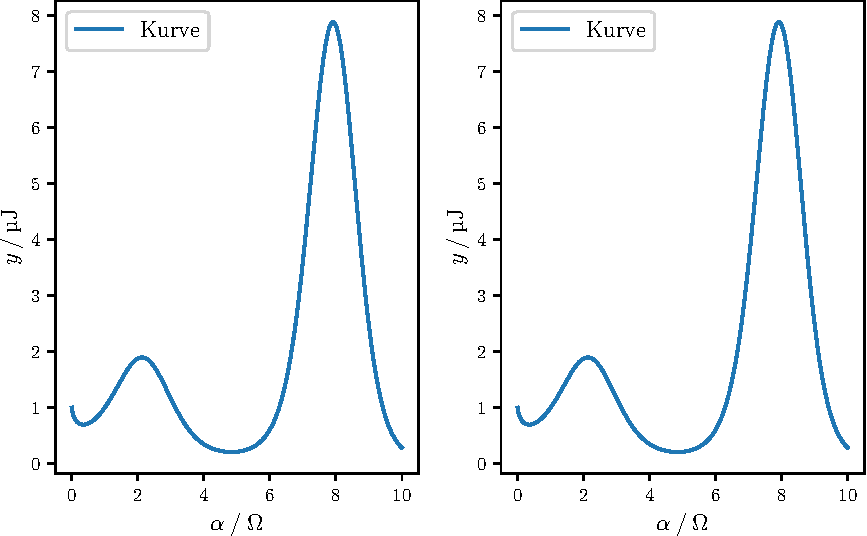
\includegraphics{plot.pdf}
%  \caption{Plot.}
%  \label{fig:plot}
%\end{figure}